\documentclass[tikz, border=10pt]{standalone}
\usepackage{tikz}
\usepackage{amsmath}
\usetikzlibrary{shapes, calc, backgrounds}

\begin{document}
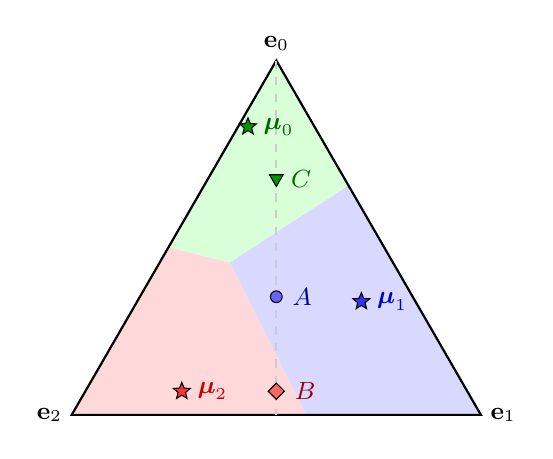
\begin{tikzpicture}[scale=0.6, font=\sffamily]

    % --- 1. Define Coordinates ---
    
    % The Triangle Vertices (Simplex)
    \coordinate (Top) at (0, 5);          
    \coordinate (Right) at (4.33, -2.5);  
    \coordinate (Left) at (-4.33, -2.5);  

    % The Prototypes (Stars)
    \coordinate (Mu0) at (-0.6, 3.6);    % Green (Top)
    \coordinate (Mu1) at (1.8, -0.1);    % Blue (Middle-Right)
    \coordinate (Mu2) at (-2.0, -2.0);   % Red (Bottom-Left)

    % The Data Points
    \coordinate (C) at (0, 2.5);   % Top Data
    \coordinate (A) at (0, 0);     % Middle Data
    \coordinate (B) at (0, -2.0);  % Bottom Data

    % --- 2. Background Regions (Voronoi Clipping) ---
    % Note: We draw these first so they are behind everything else
    
    % Region 0 (Green)
    \begin{scope}
        \clip (Top) -- (Right) -- (Left) -- cycle; 
        \path (Mu0) -- (Mu1) coordinate[midway] (M01);
        \clip ($(M01)!20cm!90:(Mu1)$) -- ($(M01)!20cm!-90:(Mu1)$) -- ($(M01)!20cm!180:(Mu1)$) -- cycle;
        \path (Mu0) -- (Mu2) coordinate[midway] (M02);
        \clip ($(M02)!20cm!90:(Mu2)$) -- ($(M02)!20cm!-90:(Mu2)$) -- ($(M02)!20cm!180:(Mu2)$) -- cycle;
        \fill[green!15] (-5,-5) rectangle (5,5);
    \end{scope}

    % Region 1 (Blue)
    \begin{scope}
        \clip (Top) -- (Right) -- (Left) -- cycle;
        \path (Mu1) -- (Mu0) coordinate[midway] (M10);
        \clip ($(M10)!20cm!90:(Mu0)$) -- ($(M10)!20cm!-90:(Mu0)$) -- ($(M10)!20cm!180:(Mu0)$) -- cycle;
        \path (Mu1) -- (Mu2) coordinate[midway] (M12);
        \clip ($(M12)!20cm!90:(Mu2)$) -- ($(M12)!20cm!-90:(Mu2)$) -- ($(M12)!20cm!180:(Mu2)$) -- cycle;
        \fill[blue!15] (-5,-5) rectangle (5,5);
    \end{scope}

    % Region 2 (Red)
    \begin{scope}
        \clip (Top) -- (Right) -- (Left) -- cycle;
        \path (Mu2) -- (Mu0) coordinate[midway] (M20);
        \clip ($(M20)!20cm!90:(Mu0)$) -- ($(M20)!20cm!-90:(Mu0)$) -- ($(M20)!20cm!180:(Mu0)$) -- cycle;
        \path (Mu2) -- (Mu1) coordinate[midway] (M21);
        \clip ($(M21)!20cm!90:(Mu1)$) -- ($(M21)!20cm!-90:(Mu1)$) -- ($(M21)!20cm!180:(Mu1)$) -- cycle;
        \fill[red!15] (-5,-5) rectangle (5,5);
    \end{scope}

    % --- 3. Draw Boundaries (Bisector Lines) ---
    % \begin{scope}
    %     \clip (Top) -- (Right) -- (Left) -- cycle;
    %     \draw[thick, green!50!black] ($(M01)!10cm!90:(Mu1)$) -- ($(M01)!10cm!-90:(Mu1)$);
    %     \draw[thick, blue!50!black] ($(M12)!10cm!90:(Mu2)$) -- ($(M12)!10cm!-90:(Mu2)$);
    %     \draw[thick, red!50!black] ($(M02)!10cm!90:(Mu2)$) -- ($(M02)!10cm!-90:(Mu2)$);
    % \end{scope}

    % --- 4. Main Triangle Frame & Blind Spot Line ---
    \draw[thick] (Top) -- (Right) -- (Left) -- cycle;
    \draw[dashed, gray!40, thick] (0, 5) -- (0, -2.5);

    % --- 5. Labels ---
    \node[above, font=\small] at (Top) {$\mathbf{e}_0$};
    \node[right, font=\small] at (Right) {$\mathbf{e}_1$};
    \node[left, font=\small] at (Left) {$\mathbf{e}_2$};

    % --- 6. Prototypes (Stars) ---
    \node[star, star points=5, star point ratio=2.25, fill=green!60!black, draw=black, inner sep=1pt] (Star0) at (Mu0) {};
    \node[right, green!40!black, font=\small\bfseries] at (Star0.east) {$\boldsymbol{\mu}_0$};
    
    \node[star, star points=5, star point ratio=2.25, fill=blue!80, draw=black, inner sep=1pt] (Star1) at (Mu1) {};
    \node[right, blue!80!black, font=\small\bfseries] at (Star1.east) {$\boldsymbol{\mu}_1$};
    
    \node[star, star points=5, star point ratio=2.25, fill=red!80, draw=black, inner sep=1pt] (Star2) at (Mu2) {};
    \node[right, red!80!black, font=\small\bfseries] at (Star2.east) {$\boldsymbol{\mu}_2$};

    % --- 7. Data Points ---
    % C (True: 0)
    \node[regular polygon, regular polygon sides=3, rotate=180, fill=green!60!black, draw=black, inner sep=1pt] (NodeC) at (C) {};
    \node[right, green!40!black, font=\small\bfseries] at (NodeC.west) {$C$};

    % A (True: 1)
    \node[circle, fill=blue!60, draw=black, inner sep=1.5pt] (NodeA) at (A) {};
    \node[right, blue!60!black, font=\small\bfseries] at (NodeA.east) {$A$};

    % B (True: 2)
    \node[diamond, fill=red!60, draw=black, inner sep=1.5pt] (NodeB) at (B) {};
    \node[right, red!60!black, font=\small\bfseries] at (NodeB.east) {$B$};

    % % --- 8. Legend ---
    % \matrix [draw, fill=white, fill opacity=0.9, anchor=south east, nodes={scale=0.8, anchor=west}] at (Right) {
    %     \node [regular polygon, regular polygon sides=3, rotate=180, fill=green!60!black, inner sep=1.5pt, label=right:Class 0] {}; \\
    %     \node [circle, fill=blue!60, inner sep=2pt, label=right:Class 1] {}; \\
    %     \node [diamond, fill=red!60, inner sep=2.5pt, label=right:Class 2] {}; \\
    %     \node [star, star points=5, fill=black, inner sep=2pt, label=right:Prototypes] {}; \\
    % };

\end{tikzpicture}
\end{document}